% Reading, Not Reasoning — short paper (arXiv preprint style, self-contained)
% Compile: pdflatex paper.tex && bibtex paper && pdflatex paper.tex && pdflatex paper.tex
\documentclass[11pt]{article}

\usepackage[margin=1in]{geometry}
\usepackage[T1]{fontenc}
\usepackage[utf8]{inputenc}
\usepackage{microtype}
\usepackage{amsmath,amssymb}
\usepackage{booktabs}
\usepackage{graphicx}
\usepackage{xcolor}
\usepackage{enumitem}
\usepackage[round,sort]{natbib}
\usepackage[colorlinks=true,linkcolor=blue!60!black,citecolor=blue!60!black,urlcolor=blue!60!black]{hyperref}
\usepackage{caption}
\captionsetup{font=small,labelfont=bf}

\emergencystretch=1.5em

\newcommand{\corrupt}{\textsc{corrupt}}
\newcommand{\shuffle}{\textsc{shuffle}}
\newcommand{\regimeone}{R1}
\newcommand{\regimetwo}{R2}

\title{\bf Reading, Not Reasoning: A Causal Faithfulness Audit of\\ Chain-of-Thought in Distilled Chart-and-Table VLMs}

\author{%
  Ruihan Su\thanks{Draft of 2026-06-26. All numbers regenerate from the project's append-only result store; see \S\ref{sec:repro}.}\\
  Sun Yat-sen University\\
  \texttt{surh6@mail2.sysu.edu.cn}
}
\date{}

\begin{document}
\maketitle

\begin{abstract}
Many multimodal systems try to compress an agentic visual reasoning trajectory into a single tool-free VLM forward pass. We ask what such distillation actually transfers. Across chart and table QA, chain-of-thought (CoT) SFT reliably improves accuracy at high power (ChartQA 32B: $.725\!\to\!.795$, $p{=}6.9{\times}10^{-5}$; TabMWP 32B: $.835\!\to\!.973$, $p{=}2.1{\times}10^{-12}$). The headline figure, however, shows the accuracy gain moving horizontally while causal faithfulness stays pinned at $F\!\approx\!0$, where $F=\mathrm{flip}_{\corrupt}-\mathrm{flip}_{\shuffle}$. The answer-time information source is usually the easiest readable source, not the emitted arithmetic step: models re-read visible charts/tables (ChartQA snap-to-true .98/.82; TabMWP .97), reconstruct natural-image counts from redundant enumerations (follow 0/345 present, 1/345 masked), or copy the chain's final conclusion in a shortcut-removing FinQA curriculum (operand-follow 0/172 at 8B and 0/175 at 32B). We therefore frame the result as a regime-dependent audit of where the causal work sits: visual evidence, redundant text, or conclusion copying. Accuracy-only internalization claims conflate these regimes; causal probes separate reading from load-bearing reasoning.
\end{abstract}

\section{Introduction}
\label{sec:intro}

Agentic VLM systems---iterative frame retrieval, self-reflection, critic-orchestrated re-reading, visual tool use---often improve accuracy, but their inference-time tools are expensive. A natural compression step is to convert an expert trajectory into a written rationale or latent trace and fine-tune a VLM to execute one forward pass at test time \citep{vpd,chartpali,pearl,zoomingwithoutzooming,locus}. Two assumptions are easy to blur:

\begin{description}[leftmargin=2.2em,itemsep=2pt]
  \item[A1 (headroom).] Holding visual evidence fixed, the agent's \emph{reasoning} (not its frame selection) beats the base model's single forward pass, so there is something type-1 (single-forward-doable) to internalize.
  \item[A2 (faithfulness).] When distillation lifts accuracy, the student's emitted CoT carries the causal work rather than merely recording, paraphrasing, or revealing an answer found elsewhere.
\end{description}

We test both. For A1 we run a multi-seed, paired-bootstrap \textbf{variance gate} over dataset $\times$ model $\times$ agentic-method cells, with label audit and power analysis. For A2 we adapt Lanham-style interventions \citep{lanham2023}: \corrupt{} one numeric intermediate, compare against \shuffle{} and other controls, force the model to answer, and record whether the final answer snaps back to the true value, follows the injected value, or goes elsewhere. The key distinction is not whether an intervention can ever perturb a model, but whether a falsified on-path value is more causal than controls under the same information regime.

\paragraph{Contributions.}
\begin{enumerate}[leftmargin=1.6em,itemsep=2pt]
  \item A variance-gated map over video, chart, and table regimes: agentic reflection over fixed evidence gives no reliable positive headroom, while static charts/tables provide high-power cells where CoT SFT truly improves single-pass accuracy.
  \item A causal faithfulness battery showing \textbf{accuracy--faithfulness decoupling}: ChartQA SFT gains of $+6.5$--$+7.0$ points and TabMWP gains of $+9.8$--$+13.8$ points coexist with $F\le 0$ and near-zero follow rates.
  \item A regime account of the answer-time information source: charts/tables are answered by re-reading visible evidence, natural-image counting by reconstructing from redundant enumerations, and shortcut-removing FinQA curricula by copying the chain's conclusion.
  \item A preregistered constructive test: even gold-program and text-teacher curricula that remove single-cell shortcuts raise accuracy but do not install load-bearing input-operand computation.
\end{enumerate}

\section{Related Work}
\label{sec:related}

\paragraph{Internalizing visual reasoning.}
Visual Program Distillation \citep{vpd}, chart-specific rationale transfer \citep{chartpali,chartr1}, latent trajectory learning \citep{pearl,capimagine2026}, and region-to-image or local-cue distillation \citep{zoomingwithoutzooming,locus} all aim to move work that previously required tools, crops, or expert traces into a cheaper model or inference path. These papers mainly validate the transfer by answer accuracy, sometimes with attention or qualitative trace analysis. Our question is narrower: after a no-tool VLM emits a discrete rationale, is the emitted intermediate value an answer-carrying state, or is it an artifact of a successful read?

\paragraph{CoT faithfulness and visual-agent faithfulness.}
Text-LLM faithfulness work shows that rationale scaffolds can be made more explicitly faithful \citep{lyu2023}, that plausible rationales can omit true decision drivers \citep{turpin2023}, that larger models can produce less answer-dependent CoT \citep{lanham2023}, and that filler tokens can support hidden computation independent of human-readable steps \citep{pfau2024}. Two critiques matter for our design: unlearning or deletion can measure contextual robustness rather than load-bearing computation \citep{tutek2025}, and multiple-choice option bias can make some faithfulness metrics look like disguised accuracy \citep{bentham2024}. In multimodal settings, recent audits target different objects: visual-thinking agents may ignore visual evidence \citep{visualthinking2025}, CodeV perturbs tool-output images rather than internalized CoT tokens \citep{codev}, and latent imagination work studies continuous intermediate states \citep{capimagine2026}. We therefore position our audit by object and mechanism: discrete CoT emitted by a distilled, single-forward VLM, evaluated with controls that separate re-reading, redundancy, and conclusion copying.

\paragraph{Why charts and tables.}
Chart and table QA are useful because the same task mixes visual extraction and numerical reasoning. ChartQA \citep{chartqa}, TabMWP \citep{tabmwp}, CharXiv \citep{charxiv}, ChartMuseum \citep{chartmuseum}, chart-noise stress tests \citep{chartnoise}, and perception-bottleneck analyses \citep{perceptionbottleneck} all point to a persistent ambiguity: an accuracy improvement can come from reading values better, computing with them better, or both. Our experiments exploit that ambiguity instead of hiding it. By masking images, falsifying on-path operands, and comparing chart/table with natural-image counting, we ask which representation the answer actually reads from at the final step.

\section{Experimental Setup}
\label{sec:setup}

\paragraph{Tasks.}
\emph{NExT-GQA} \citep{nextgqa} (short-video MCQ with grounding ground truth; 16 uniformly sampled frames; we verify 47 clean, evidence-visible pilot cases), \emph{CLEVRER} \citep{clevrer} (collision reasoning), \emph{ChartQA} \citep{chartqa} (400 held-out open numeric questions, image-disjoint from SFT train images), \emph{TabMWP} \citep{tabmwp} (400 rendered-table, free-response numeric cases), TallyQA-complex natural-image counting (400 open integer questions), and FinQA rendered tables for the preregistered curriculum probe.

\paragraph{Models.}
Qwen3-VL 4B / 8B / 30B-A3B (MoE) / 32B (dense) \citep{qwen3vl}; InternVL3-8B \citep{internvl3} (fixed-resolution ViT; cross-family control); Penguin-VL 2B/8B \citep{penguinvl} (LLM-based vision encoder with temporal token compression; cross-\emph{paradigm} control). All models are served locally; the orchestrator/critic is a text-only LLM, never a stronger VLM teacher for the video gates.

\paragraph{Agentic methods (frames held fixed = the type-1 isolation).}
\textsc{self-reflect} (2-turn tool-free self-re-examination over the same frames); \textsc{orch-blind} (a text critic poses sub-questions, the VLM is the eyes, the critic integrates); \textsc{orch-sighted} (a 32B-VLM critic that can re-read the image). Frame retrieval is deliberately excluded: it changes the evidence (type-2) and cannot be internalized into a fixed-input forward pass.

\paragraph{Statistics.}
$K$ seeds per gate cell ($K{=}10$ for 4B/8B NExT, 6 for 32B, 3--5 elsewhere); paired bootstrap 95\% CIs on agentic net (gain $-$ loss); McNemar exact tests for paired SFT deltas; and an explicit power table. The original video pilot remains underpowered ($n{=}47$, minimum detectable net about 25 points at 80\% power), so video nulls are stated as no reliable fixed-evidence headroom. The ChartQA expansion closes the main power gap: at $n{=}400$, minimum detectable net is about 8--9 points, and the observed paired SFT gains have 66 and 46 discordant pairs at 8B/32B.

\paragraph{Robustness to known confounds.}
We do not claim the \corrupt{} intervention itself is new; it is useful only as part of a controlled battery. To address the ``contextual faithfulness'' concern \citep{tutek2025}, we compare \corrupt{} against \shuffle{}, paraphrase, filler-token, deletion, truncation, image-mask, and a snap/follow/other readout that asks whether the final answer follows the injected value. To address disguised-accuracy and option-bias concerns \citep{bentham2024}, the main faithfulness substrates are free-response numeric QA rather than multiple choice. To avoid reporting a probe artifact as mechanism, we treat a positive corruption flip as insufficient by itself; the headline evidence is convergence across controls and regimes.

\section{Result I: The Two-Regime Map}
\label{sec:map}

\begin{figure}[t]
\centering
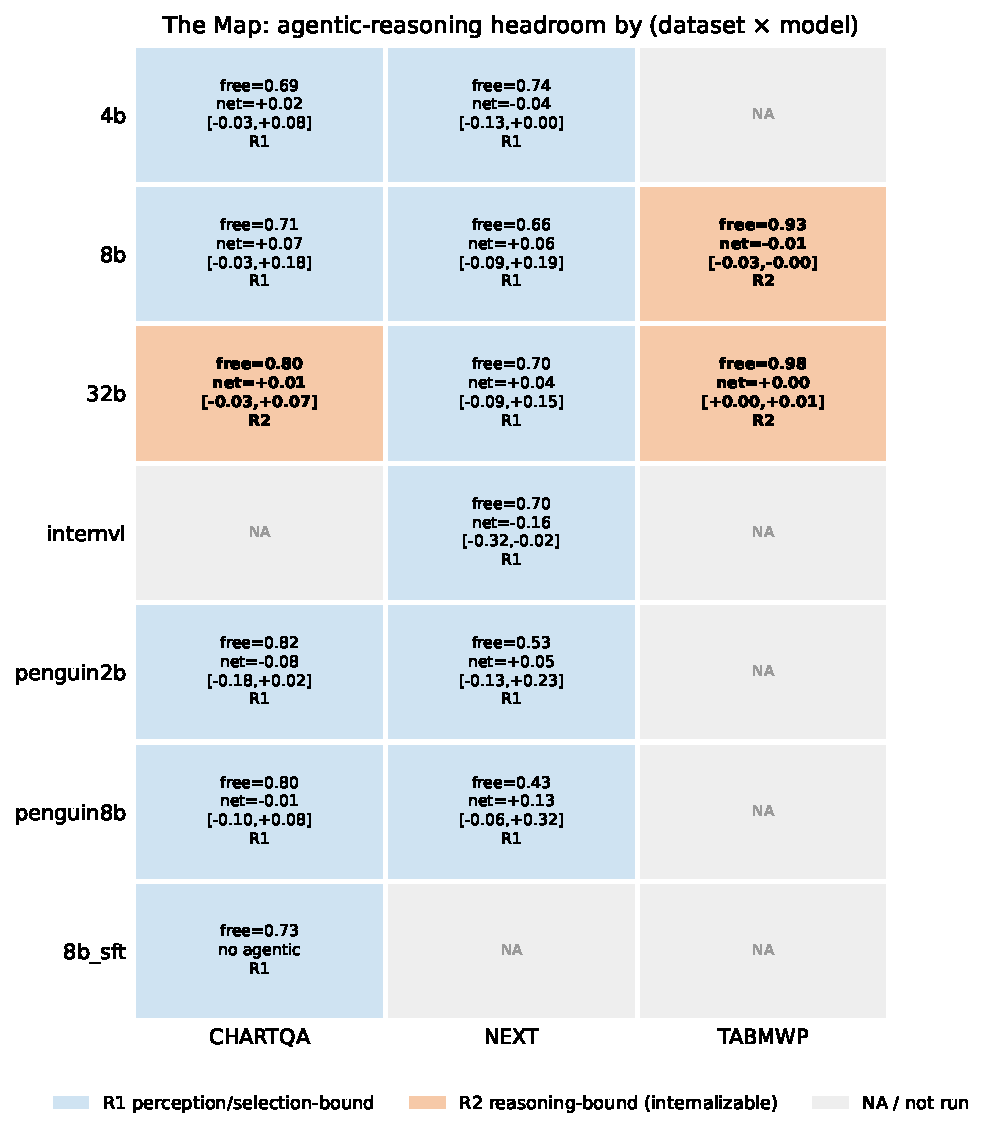
\includegraphics[width=0.6\textwidth]{figures/fig_map.pdf}
\caption{\textbf{The map.} Variance-gated agentic-reasoning headroom per (dataset $\times$ model); cell colour encodes regime. Reasoning-bound cells now include 32B ChartQA and 8B/32B TabMWP, where perception is largely solved and residual errors are arithmetic/table reasoning. Annotations are free-form accuracy, best-agentic net and paired-bootstrap CI. Regenerated from the result store by \texttt{scripts/build\_faithfulness\_axis.py}.}
\label{fig:map}
\end{figure}

\begin{table}[t]
\centering
\footnotesize
\setlength{\tabcolsep}{4.5pt}
\caption{The variance-gated map. ``Best agentic net'' is the best available fixed-evidence agentic method vs.\ free-form, pooled over seeds. No cell shows reliable positive agentic headroom; reliably negative cells are \textbf{bold}. \regimeone{} = perception/selection-bound; \regimetwo{} = reasoning-bound for SFT/audit.}
\label{tab:map}
\resizebox{\textwidth}{!}{%
\begin{tabular}{@{}llllc@{}}
\toprule
Dataset $\times$ model & Free acc & Best agentic net & Verdict & Regime \\
\midrule
NExT 4B / 8B / 32B & .74 / .66 / .70 & $-.045$ / $+.060$ / $+.039$ & within-var.\ ($K{=}10/10/6$) & \regimeone \\
NExT InternVL3-8B & .70 & orch $\mathbf{-.163}$ & \textbf{rel.\ neg.}\ (CI $[-.32,-.02]$) & \regimeone\ (family) \\
NExT Penguin 2B / 8B & .53 / .43$^{\dagger}$ & $+.050$ / $+.128$ & within-var.\ ($K{=}3$) & \regimeone\ (paradigm) \\
CLEVRER 4B--32B & .43--.50 & $\approx 0$ & $\approx$chance; tracking wall & \regimeone \\
ChartQA 4B / 8B & .685 / .708 & $+.018$ / $+.070$ & within-var. & \regimeone\ (reading) \\
ChartQA Penguin 2B / 8B & \textbf{.82} / \textbf{.80} & $-.078$ / $-.006$ & within-var.\ ($K{=}3$) & \regimeone\ (enc.\ solves) \\
\textbf{ChartQA 32B} & \textbf{.798} & $+.012$ & within-var. & \textbf{\regimetwo} \\
\textbf{TabMWP 8B / 32B} & \textbf{.928 / .980} & $\mathbf{-.014}$ / $+.003$ & \textbf{rel.\ neg.} / within-var. & \textbf{\regimetwo} \\
\bottomrule
\end{tabular}}

\smallskip
\raggedright\footnotesize $^{\dagger}$Penguin-8B on NExT ran frame-starved at 2 frames (memory limit); not comparable to 16-frame cells.
\end{table}

Table~\ref{tab:map} summarizes the gate. The map is not an argument that charts and tables are easy; it says the visual read is good enough that SFT can test whether a written chain carries the remaining arithmetic.

\paragraph{(a) No cell shows reliable agentic headroom; the reliable effects are negative.}
Across all fixed-evidence cells, no agentic/reflective method beats single-forward outside run variance. Several cells show reliable harm: InternVL3-NExT $-16.3\%$ and TabMWP-8B self-reflection $-1.4\%$ despite a high base accuracy. Per-case dumps show a recurring failure mode: a second read often revises a correct first read into a contradiction. Multi-step orchestration adds failure points unless the added step changes the evidence itself.

\paragraph{(b) The retraction.}
Our single-seed sweep had one positive headline: 8B-NExT orchestrated reflection $+8\%$. Ten seeds reduce it to $\mathbf{+0.9\%}$ with sign flips. The variance source is the critic's stochastic sub-questions, not the VLM's decoding. Single-seed agentic gains at this $n$ are not evidence.

\paragraph{(c) Why regime 1 is perceptual: converging probes.}
On the 18 8B-NExT free-form errors, giving the model the \emph{ground-truth} frames at maximum resolution recovers only 4/18 (22\%); a near-oracle (32B captions of GT frames $\to$ text-LLM reasons) recovers 6/18 (33\%). Two-thirds of the failure surface is unreachable by any reasoning-over-fixed-frames intervention. The sighted-critic ablation sharpens the mechanism: a 32B sighted critic trends positive on every seed on \emph{charts} ($+.070$, where the wall is re-readable values) but not on \emph{video} ($+.060$, CI crossing 0, where the wall is temporal localization that re-reading the same 16 frames cannot fix).

\paragraph{(d) The encoder-paradigm result.}
Penguin-VL's LLM-based encoder lifts small-model chart reading to \textbf{.82 (2B)}---matching Qwen-32B (.80) and above Qwen-8B (.71). Yet the temporal-video wall is unmoved (Penguin-2B NExT .53) and agentic nets stay unreliable. The regime structure is a property of the task and evidence access, not just parameter count.

\section{Result II: Internalization Works in Regime 2---by Accuracy}
\label{sec:sft}

In the reasoning-bound cells, we run the actual distillation. A Qwen3-VL teacher generates step-by-step rationales; answer-consistency filtering keeps high-quality traces; LoRA/QLoRA SFT trains a single-forward student. All reported evaluation sets are image-disjoint from training and use open numeric grading.

\begin{itemize}[leftmargin=1.6em,itemsep=2pt]
  \item \textbf{ChartQA, $n{=}400$:} 8B $.713 \to \mathbf{.778}$, net $+6.5$ points, CI $[+2.5,+10.5]$, McNemar $p{=}0.0021$; 32B $.725 \to \mathbf{.795}$, net $+7.0$ points, CI $[+3.8,+10.3]$, McNemar $p{=}6.9{\times}10^{-5}$. The original 32B $n{=}60$ pilot had only four discordant pairs; the expanded evaluation has 37 gains vs.\ 9 losses.
  \item \textbf{TabMWP, $n{=}400$:} 8B $.865 \to \mathbf{.963}$, net $+9.8$ points, McNemar $p{=}2.9{\times}10^{-9}$; 32B $.835 \to \mathbf{.973}$, net $+13.8$ points, McNemar $p{=}2.1{\times}10^{-12}$.
\end{itemize}

Thus the paper is not a null-result critique of SFT. The accuracy gains are real, paired, and adequately powered on static chart/table substrates. The remaining question is what mechanism those gains bought.

\section{Result III: The Causal Probe---the Gain Is Reading, Not Reasoning}
\label{sec:probe}

\begin{figure}[t]
\centering
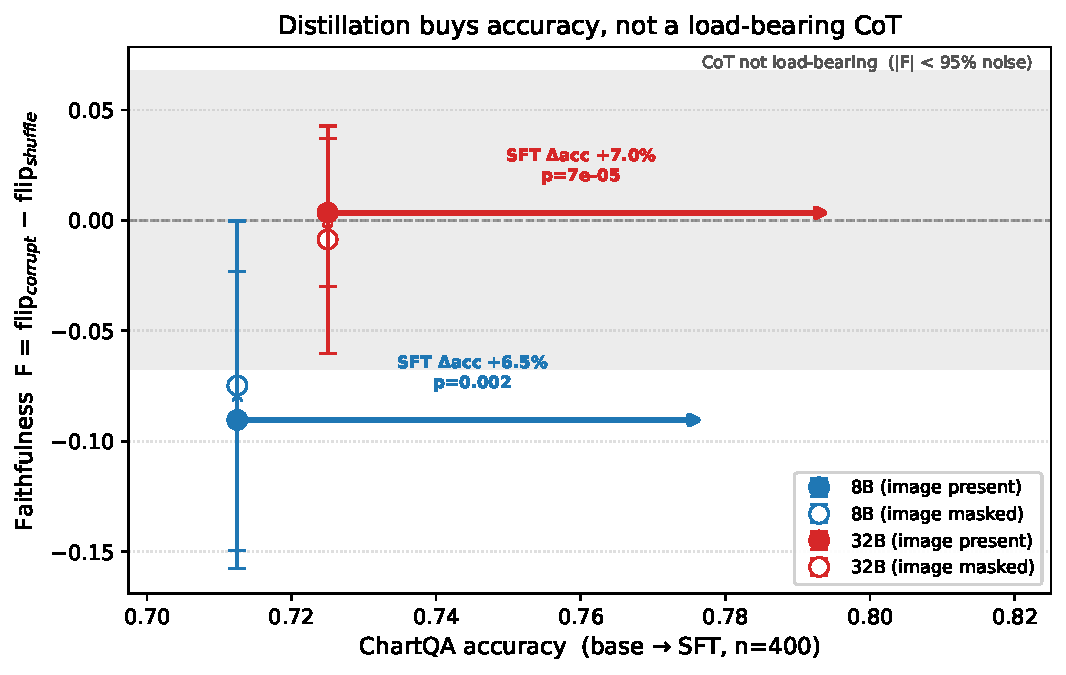
\includegraphics[width=\columnwidth]{figures/fig_decoupling.pdf}
\caption{\textbf{Accuracy $\perp$ faithfulness.} CoT distillation lifts ChartQA accuracy by $+6.5$--$7.0\%$ (McNemar $p\!\le\!.002$; horizontal arrows), yet the causal CoT metric stays on the $F\!\approx\!0$ band ($F=\text{flip}_{\corrupt}-\text{flip}_{\shuffle}$): corrupting a numeric intermediate flips the answer no more than shuffling the CoT. Hollow markers show image-masked controls. $F$ is measured on the base model; error bars are $95\%$ binomial CIs. Regenerated from the result store by \texttt{scripts/build\_faithfulness\_axis.py}.}
\label{fig:decoupling}
\end{figure}

For every correctly answered case with an emitted CoT, we intervene on the rationale and force-continue to a final answer. If a numeric intermediate carries the computation, \corrupt{} should flip more often than \shuffle{}, and the final answer should follow the injected value rather than snap back to the original truth. Table~\ref{tab:probe} reports the high-power ChartQA and TabMWP cells.

\begin{table}[t]
\centering
\small
\caption{Causal CoT-intermediate probe on chart/table SFT cells. ``Flip'' = final answer changes after the intervention. ``Snap'' = answer returns to the true chart/table value after \corrupt{}; ``follow'' = answer follows the injected value. A load-bearing chain requires \corrupt{} $>$ controls and nontrivial follow.}
\label{tab:probe}
\resizebox{\textwidth}{!}{%
\begin{tabular}{@{}llccccc@{}}
\toprule
Dataset/model & Condition & $n$ & \corrupt & \shuffle & snap & follow \\
\midrule
ChartQA 8B  & present & 321 & .212 & .302 & .816 & .031 \\
ChartQA 32B & present & 318 & .051 & .047 & .981 & .016 \\
TabMWP 8B   & present & 385 & .034 & .145 & .971 & .008 \\
TabMWP 32B  & present & 389 & .033 & .072 & .969 & .015 \\
TabMWP 8B   & masked  & 385 & .278 & .299 & .722 & .088 \\
TabMWP 32B  & masked  & 389 & .075 & .103 & .928 & .039 \\
\bottomrule
\end{tabular}}
\end{table}

Four findings follow.

\begin{enumerate}[leftmargin=1.6em,itemsep=2pt]
  \item \textbf{ChartQA and TabMWP agree.} In every present-image/table cell, $\corrupt{}\leq\shuffle{}$ up to sampling noise. The model usually snaps back to the true value and almost never follows the injected value. TabMWP is the cleanest case: despite large SFT gains, follow is .008/.015 at 8B/32B.
  \item \textbf{The gain subset itself is reading.} On TabMWP cases newly solved by SFT, corrupting the CoT flips 0/40 8B gains and 1/57 32B gains; follow is 1/40 and 0/57. The new correct answers are not being computed from the falsified written arithmetic.
  \item \textbf{Masking diagnoses the information source.} On tables, masking the image raises flip and ``other'' errors sharply, especially for 8B, but follow remains small. When the table is visible, the final answer step re-reads and recomputes from the table; when the table is removed, the model often fabricates rather than faithfully using the bad chain.
  \item \textbf{Other interventions point the same way.} Paraphrase behaves like \corrupt{} (e.g., 32B ChartQA present .053 vs.\ .051), filler/truncation/deletion mainly test format and token-budget sensitivity, and early-answering curves are monotone. The conclusion is carried by the whole battery, not by a single corruption statistic.
\end{enumerate}

\section{Result IV: Regime Dependence and a Constructive Failure}
\label{sec:regime}

\paragraph{Natural-image counting.}
To test whether the chart/table result is a chart artifact, we run a preregistered TallyQA-complex counting probe on base Qwen3-VL-8B/32B, with no chart adapter. This is a genuinely perception-bottlenecked natural-image regime (free-form accuracy .415/.448). Yet the emitted CoT's numeric content is again not load-bearing: across scales, follow is 0/345 with the image present and 1/345 when masked. Even when \corrupt{} hits the count token itself, follow is 0/103 present and 1/103 masked. The model reconstructs the answer from redundant enumeration in the text, so masking the image is almost inert. This is the same reading-not-reasoning pattern with a different readable source: not the image, but the redundant chain.

\paragraph{Shortcut-removing curriculum.}
As a constructive counter-test, we train on rendered FinQA tables filtered to require multi-step, multi-cell arithmetic with a gold-program-verified flippable operand. The curriculum uses a deterministic gold-program teacher and a matched vanilla control; a text-teacher arm repeats the test with fluent answer-conditioned rationales. Accuracy rises substantially (8B: .080 base $\to$ .582 vanilla $\to$ .674 curriculum; 32B: .123 $\to$ .659 $\to$ .682). But the targeted probe still finds no load-bearing operand use: changing a verified on-path \emph{input} operand yields follow 0/172 for the 8B curriculum and 0/175 for the 32B curriculum. When the chain's final conclusion is consistently rewritten to the recomputed value, the model follows it in 96--97\% of cases. The mechanism is conclusion copying, not recomputation from operands. Thus even a shortcut-removing curriculum can improve accuracy without installing a load-bearing written chain.

\section{Discussion and Limitations}
\label{sec:discussion}

\paragraph{Implications.}
(i) Claims of ``internalizing agentic reasoning'' need causal audits. Significant accuracy gains are compatible with re-reading visual evidence, reconstructing from redundant rationale text, or copying the rationale's conclusion. (ii) The load-bearing locus is regime-dependent: answer-time evidence can live in pixels, in redundant text, or in a conclusion line. A single CoT faithfulness score without information-source controls is under-specified. (iii) Fixed-evidence reflection is a poor substitute for perception routing; if the agent's true advantage is frame/region selection, single-forward distillation must be evaluated as perceptual transfer rather than reasoning transfer.

\paragraph{Limitations.}
The video gate remains small ($n{=}47$) and is used only to motivate the fixed-evidence boundary; the high-power causal claims are on ChartQA/TabMWP/TallyQA/FinQA. The 32B students use QLoRA/NF4 rather than full bf16 fine-tuning. The main teacher family is Qwen3-VL, although the FinQA text-teacher arm reduces a format-specific teacher concern. Corrupting one numeric token is a sensitivity lower bound; we therefore report it only with shuffle/paraphrase/filler/truncation, image masking, snap/follow/other classification, and targeted gold-program operand tests.

\section{Conclusion}
\label{sec:conclusion}

We set out to compress tool-scaffolded visual reasoning into one forward pass and to verify what moved. The answer is not a blanket dismissal of CoT or of distillation: SFT works, often strongly. The causal result is more specific. In these chart, table, natural-counting, and rendered-FinQA regimes, the answer reads from the easiest available source: pixels, redundant enumerations, or the chain's final conclusion. Accuracy can move while load-bearing CoT faithfulness does not. That is the audit lesson behind \emph{Reading, Not Reasoning}.

\section*{Reproducibility Statement}
\label{sec:repro}
All gate numbers regenerate from a fingerprinted, append-only result store (\texttt{results.jsonl}) via the released gate/table scripts; SFT, merge, battery, curriculum, and probe scripts are included. The variance gate, label audit, ChartQA/TabMWP builders, power table, faithfulness figures, N3 natural-counting probe, and N1 targeted curriculum probe each correspond to one script with fixed seeds or saved artifacts.

\bibliographystyle{plainnat}
\bibliography{references}

\end{document}
